\subsection{Sets construction}

Now, to make it reasonable for a complete ordered field $\mathbb{F}$ to be isomorphic to our known $\mathbb{R}$, we need to start shaping it using the parts that make it up. Think of $\mathbb{R}$ as the joint set of irrational and rational numbers, which contain the other types of number as well.

\begin{figure}[h]
\centering
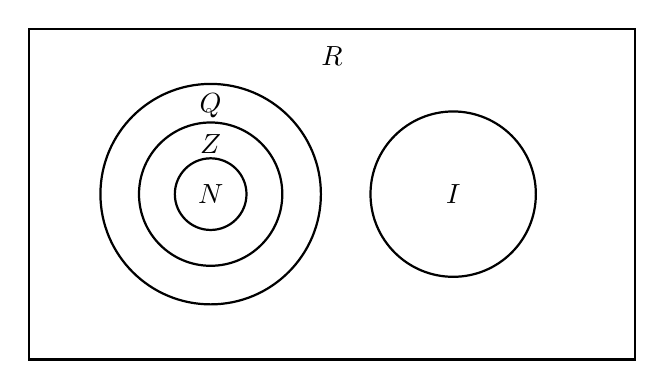
\begin{tikzpicture}[scale=0.7]
    % Real numbers rectangle (outermost)
    \draw[thick] (-5.5,-3) rectangle (5.5,3);
    \node at (0, 2.5) {$\mathbb{R}$};
    
    % Rational numbers circle (left side)
    \draw[thick] (-2.2,0) circle (2cm);
    \node at (-2.2, 1.6) {$\mathbb{Q}$};
    
    % Integers circle
    \draw[thick] (-2.2,0) circle (1.3cm);
    \node at (-2.2, 0.9) {$\mathbb{Z}$};
    
    % Natural numbers circle (innermost)
    \draw[thick] (-2.2,0) circle (0.65cm);
    \node at (-2.2, 0) {$\mathbb{N}$};
    
    % Irrational numbers circle (right side, disjoint)
    \draw[thick] (2.2,0) circle (1.5cm);
    \node at (2.2, 0) {$\mathbb{I}$};
    
\end{tikzpicture}
\captionsetup{width=0.8\textwidth}
\caption{\small{Hierarchy of number sets: Natural numbers ($\mathbb{N}$), Integers ($\mathbb{Z}$), Rationals ($\mathbb{Q}$), Irrationals ($\mathbb{I}$), and Real numbers ($\mathbb{R}$).}}
\label{fig:number_sets}
\end{figure}


From this idea, we need to build $\mathbb{N_F}$, $\mathbb{Z_F}$, $\mathbb{Q_F}$ and $\mathbb{I_F}$ to finall get this $\mathbb{F}$ we want. This will all make sense in the last part of the process, and it is true that it will be a bit of a hussle to construct all of it (specially $\mathbb{I_F}$ from $\mathbb{Q_F}$), but we need to go step by step.


\begin{definition}[$\mathbb{N}_{\mathbb{F}}$ by induction]
Let $\mathbb{F}$ be \textit{the} complete ordered field. Using $1_\mathbb{F}$: multiplicative neutral of $\mathbb{F}$, we declare the following element contruction:

\begin{align*}
&1_\mathbb{F} := 1_\mathbb{F}\\
&2_\mathbb{F} := 1_\mathbb{F} + 1_\mathbb{F}\\
&3_\mathbb{F} := 1_\mathbb{F} + 1_\mathbb{F} + 1_\mathbb{F}\\
\vdots\\
&n_\mathbb{F} := \sum_{1}^{n}{1_F}
\end{align*}

Finally, we define the set:
$$\mathbb{N_F} := \{1_\mathbb{F}, 2_\mathbb{F}, 3_\mathbb{F}, \dots\} = \{n_\mathbb{F}: n \in \mathbb{N} \}$$
\end{definition}

\begin{definition}[$\mathbb{Z}_\mathbb{F}$ by extension]
Within field $\mathbb{F}$, let the following:
\begin{enumerate}
\item $0_\mathbb{F}$: Additive identity
\item $-x$: Additive inverse
\end{enumerate}

We define the set:
$$\mathbb{Z_F} = \{0_\mathbb{F}\} \cup \mathbb{N_F} \cup \{-x_\mathbb{F}, \forall n_\mathbb{F} \in N_\mathbb{F}\}$$
\end{definition}

\begin{definition}[$\mathbb{Q}_\mathbb{F}$ by operation]
Within field $\mathbb{F}$, let the following:
\begin{enumerate}
\item $a \in \mathbb{F}$
\item $b^{-1}$ (multiplicative inverse of $b$) $\in \mathbb{F}$
\end{enumerate} we define the set:
$$\mathbb{Q_F} := \{\frac{a}{b}: a \in \mathbb{Z_F}, b \in \mathbb{N_F}\}$$
\end{definition}

Starting similarly to \cref{th:archimedean} (Archimedean property) we use the inductive approach to reach $\mathbb{N_F}$. Fancy but not complicated at all. Later, we just extend integers in $\mathbb{F}$ to build by $\mathbb{Z_F}$ to conclude defining $\mathbb{Q_F}$ with the result of operating arbitrary elements $a, b \in \mathbb{F}$ as $a.b^{-1}$.

Notice how we only used existent elements from $\mathbb{F}$ computed using the field's operations and nothing else. Is important to mention that you as the reader don't know yet the usage of these new sets, althought we could make a good guess.

Now comes the tricky part for us. One could think that the next steps involve 1. to prove that the irrational (in $\mathbb{F}$) is in fact buildable from $\mathbb{Q_F}$, and 2. to prove that there is a isomorphism between this result and the $\mathbb{R}$ we know.

That won't be the case. If we would go down that path, we would just be creating an arbitrary function $\Phi$ that maps a generic $\mathbb{F}$ with $\mathbb{R}$ perfectly, losing all progress we made constructing these specific sets one by one (for a reason). The real strategy here is to first prove that $\Phi$ exists and \textit{then} to try to extend this function to make it follow all expected properties in the irrationals. Buckle up.
